% \chapter{N-Fold via LP rounding} \label{platform}
\section{N-Fold via LP rounding} 

The main drawback of the augmentation algorithm is that after solving the linear relaxation, we can be arbitrarily far from the optimal solution of the IP, what means that we might need many augmentation steps. In this section we follow a different approach introduced in \cite{EISENBRAND:2020}. Intuitively, we first solve a more restricted linear relaxation which optimum is closer to the optimum of the IP. After solving this restricted linear relaxation, we can find an optimum with only one augmentation step. We first introduce this restricted linear relaxation (RLR):


\subsection{Restricted linear relaxation}

We can express the \emph{N-Fold IP} with the following equivalent block decomposition:
\begin{equation*}
    (\mathcal{N}-IP) \equiv max\{\sum (c^{(i)})^t y^{(i)} : \sum A^{(i)} y^{(i)} = b_0, y^{(i)} \in P_i, y \in \mathbb{Z}^{nt} \}
\end{equation*}
\vspace{-50pt}
\begin{center}
$P_i = \{x \in \mathbb{R}^t: B^{(i)}x = b_i, l_i \leq x \leq u_i \}, A \in \mathbb{Z}^{m \times n}$, $b_0 \in \mathbb{Z}^r$, $c_i,l_i,u_i \in \mathbb{Z}^t$
\end{center}

The classical linear relaxation (LR) is obtained by only removing the $y \in \mathbb{Z}^{nt}$ constraint, the RLR restricts also each $P_i$ to $Q_i = conv(P_i \cap \mathbb{Z}^t)$.

\begin{figure}[h]
\centering
\begin{minipage}[b]{0.45\textwidth}
    \centering
    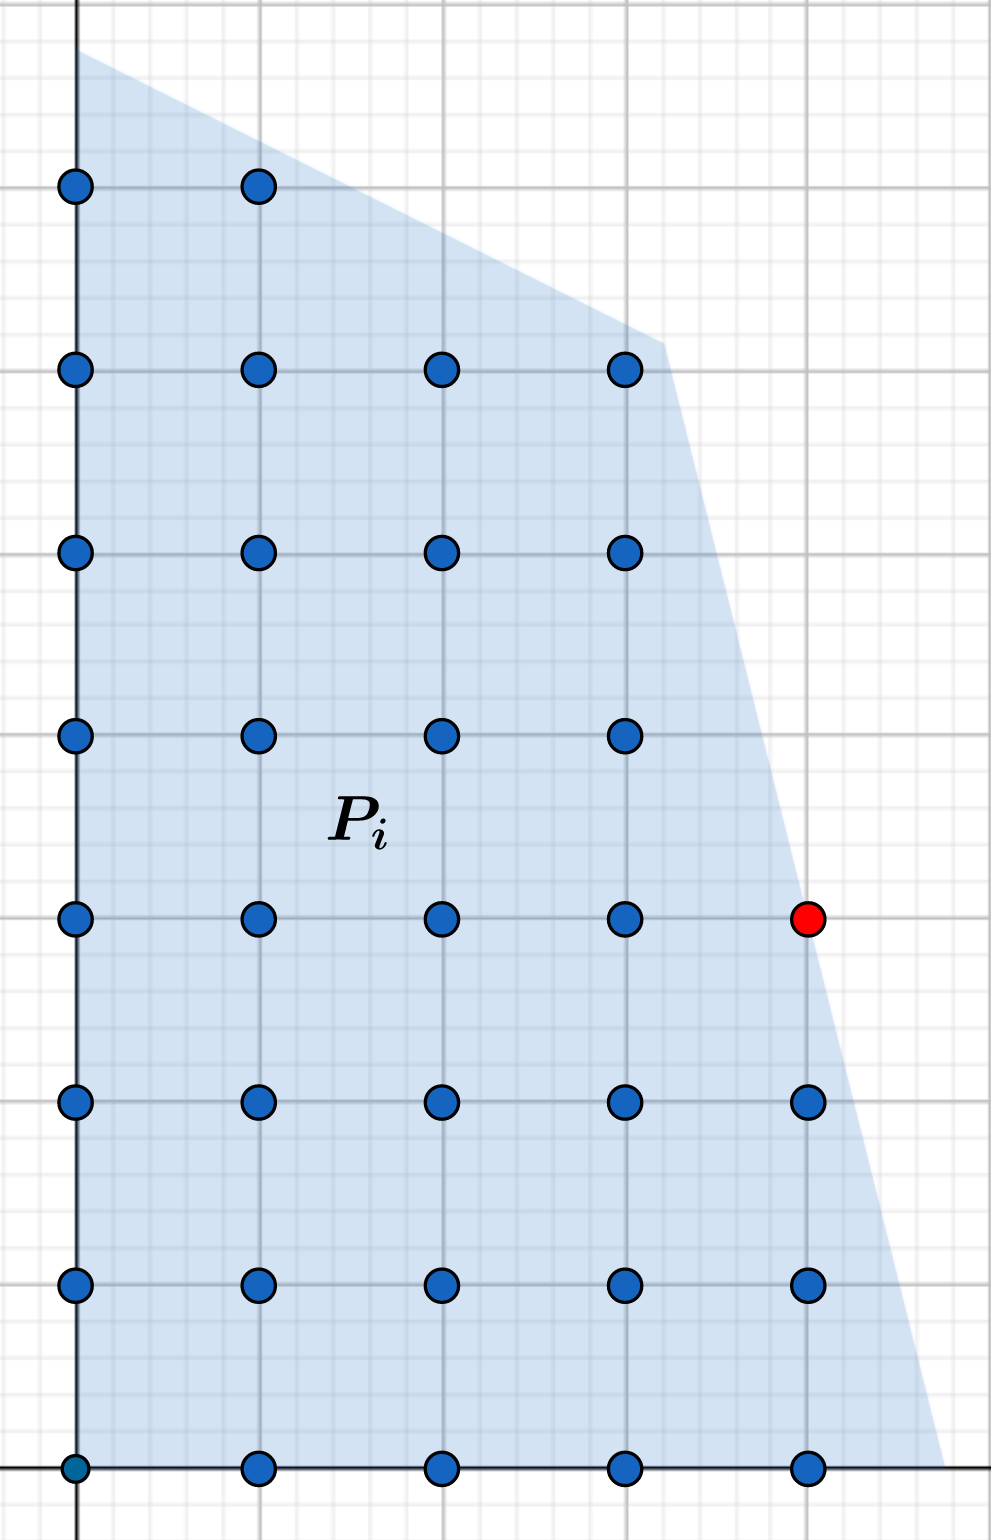
\includegraphics[width=0.9\textwidth]{images/IP(4).png}
    \caption{Linear relaxation}
\end{minipage}
\hfill
\begin{minipage}[b]{0.45\textwidth}
    \centering
    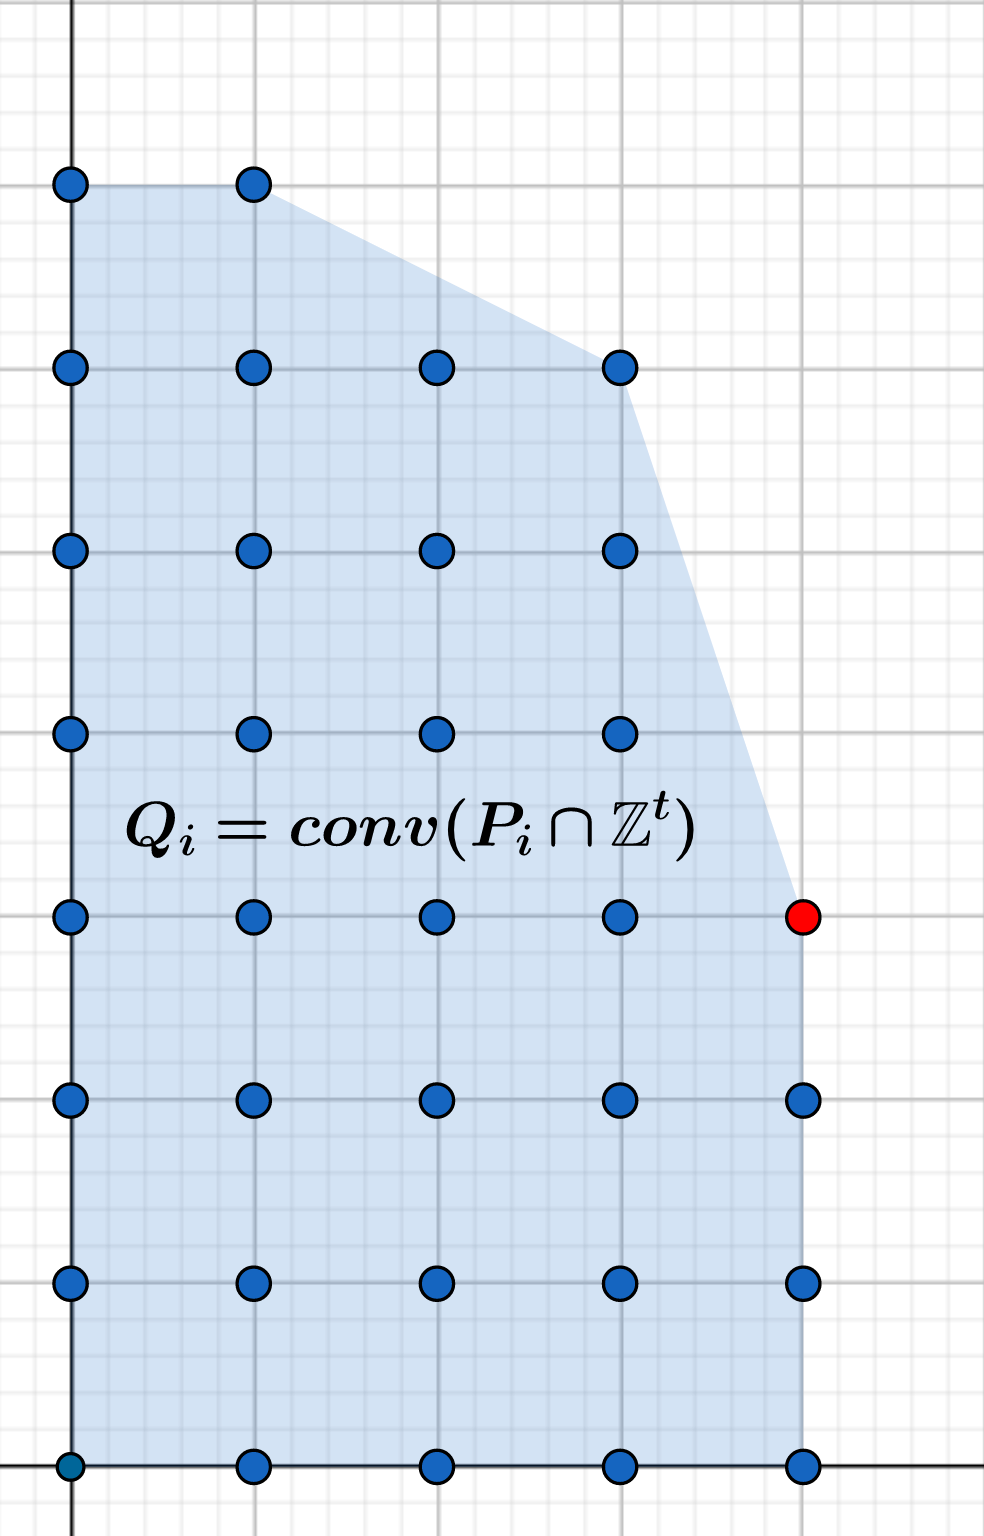
\includegraphics[width=0.9\textwidth]{images/IP(3).png}
    \caption{Restricted LR}
\end{minipage}
\end{figure}

Solving the restricted linear relaxation problem is not an easy task in practice. It was proved in \cite{EISENBRAND:2020} by applying the \emph{ellipsoid method} that it can be solved in linear time (ignoring logarithmic factors). We won't go into details of the proof here. In the following lemma and in the next ones, $\varphi$ denotes the maximum encoding length of the input and $p$ a polynomial.

\begin{lemma}[\textbf{N-Fold RLR complexity}]
    The N-Fold IP restricted linear relaxation problem can be solved in time
    \vspace{-5pt}
    \begin{equation*}
        O(nt \cdot log^2(nt) \cdot \varphi p(r) (s\Delta)^{O(s^2)})
    \end{equation*}
\end{lemma}

\vspace{-5pt}
As in the previous algorithm, solving this RLR will be the first step. We can see that the complexity of this first step has slightly increased. However, this algorithm will be more efficient thanks to the following result \cite[Section 3]{EISENBRAND:2020}:

\begin{lemma}[\textbf{N-Fold proximity to RLR}]\label{NFold_proximity_bound}
    Let $x^*$ be an optimal vertex solution of a N-Fold RLR, then there exists an optimal solution $z^*$ for the N-Fold IP verifying:  
    \vspace{-5pt}
    \begin{equation*}
        ||z^* - x^*||_1 \leq (rs\Delta)^{O(rs)}
    \end{equation*}
\end{lemma}

\vspace{-5pt}
Note that, unlike the proximity bound to the LR, which was linear in the number of variables, once fixed the order of the matrices $A_i$ and $B_i$ (parameters $r$ and $s$) the bound is constant. This, together with the dynamic program we present below, is the reason of success of our algorithm.

\subsection{Dynamic program}        

We present in this section the second and last step of our algorithm. A program which takes an optimal solution of the restricted linear relaxation and finds an optimal solution of the \emph{N-Fold IP}. The idea behind this program \cite{EISENBRAND:2020} is creating a weighted directed acyclic graph in which a longest path between two specific vertices corresponds to an optimal solution. Then, using dynamic programming we can compute a longest path in a directed acyclic graph in linear time in the number of nodes and edges. This is also the program used for proving the lemma \ref{NFold_augmentation_step_complexity}.

\begin{proposition}[\textbf{N-Fold RLR to optimum complexity}]
    Given an optimal vertex of an N-Fold RLR, the N-Fold IP can be solved in time
    \begin{equation*}
        O(nt \cdot (rs\Delta)^{O(r^2s+s^2)})
    \end{equation*}
\end{proposition}
\begin{proof}
For avoiding heavy notation, we denote $\gamma := (rs\Delta)^{O(rs)}$. First we define:

\vspace{-20pt}

\begin{equation*}
S_\ell := \{ y \in \mathbb{Z}^r: || \sum_{i=1}^\ell A_ix_i^* - y||_\infty \leq \gamma \}
\end{equation*}
        
\vspace{-10pt}        

We construct now a weighted directed acyclic graph G(V,E) with vertices

\vspace{-20pt}

\begin{equation*}
    V = \{(\ell,y) / y \in S_\ell\} \cup \{ (0,0), (n,b_0) \}
\end{equation*}

\vspace{-10pt}

and weighted edges between $(\ell-1,y)$ and $(\ell,y')$ if the following problem is feasible and, if so, we take the weight as the maximum:

\vspace{-20pt}

\begin{equation*}
    EP_\ell \equiv max\{c_\ell^tx: A_\ell x = (y'-y), B_\ell x = b_\ell, l_\ell \leq x \leq u_\ell \}
\end{equation*}

\vspace{-10pt}

Now the graph is constructed, we proof that a longest path from $(0,0)$ to $(n,b_0)$ in G(V,E) corresponds to an optimal solution of the \emph{N-Fold integer program}.

% PART 1: Point z => Path (and path cost >= c^t z)
First we prove that every feasible point $z$ verifying the proximity bound corresponds to a path from $(0,0)$ to $(n,b_0)$ and that the value of the objective function at this point is lower or equal than the path cost. Note that $z$ fulfils:

\vspace{-30pt}

\begin{align*}
    ||x^* - z||_1 \leq \gamma 
    & \implies \sum_{i=1}^\ell ||x_i^* - z_i||_1 \leq \gamma\\ 
    & \implies \sum_{i=1}^\ell ||A_i(x_i^* - z_i)||_\infty \leq \Delta \gamma = \gamma
\end{align*}

\vspace{-10pt}

%Therefore, for every feasible point z verifying the proximity bound we have:

%\vspace{-20pt}

%\begin{equation*}
%\sum_{i=1}^\ell A_ix_i^* - \gamma \leq \sum_{i=1}^\ell A_iz_i \leq \sum_{i=1}^\ell A_ix_i^* + \gamma 
%\end{equation*}
%\vspace{-5pt}

Then for every $\ell \in \{1,...,n\}$ $(\ell, \sum_{i=1}^\ell A_iz_i)$ is a vertex and $z_\ell$ is a feasible point of $EP_\ell$.  

\begin{center}
\begin{tikzpicture}[
        > = stealth, % arrow head style
        shorten > = 1pt, % don't touch arrow head to node
        auto,
        node distance = 3cm, % distance between nodes
        semithick % line style
    ]
    \tikzstyle{every state}=[
        draw = black,
        thick,
        fill = white,
        minimum size = 4mm
    ]
    \node[state, minimum size=0.8cm] (s) at (0,0) {$0$};
    
    %\node[state] (w1) at (2,2)  {$y_{11}$};
    %\node[state] (u1) at (2,0)  {$y_{12}$};
    \node (v1) at (2,-2) {$A_1z_1$};
    
    %\node (u2) at (4,0)  {$\sum_{i=1}^\ell A_ix^*$};
    \node (w2) at (4,2)  {$\sum_{i=1}^2A_iz_i$};
    %\node[state] (u2) at (4,0)  {$y_{22}$};
    %\node[state] (v2) at (4,-2) {$y_{23}$};
    
    %\node[state] (w3) at (6,2)  {$y_{31}$};
    \node (u3) at (6,0)  {$\sum_{i=1}^3A_iz_i$};
    %\node[state] (v3) at (6,-2) {$y_{33}$};
    
    \node (w4) at (8,2)  {$\sum_{i=1}^4A_iz_i$};
    %\node[state] (u4) at (8,0)  {$y_{42}$};
    %\node[state] (v4) at (8,-2) {$y_{43}$};
    
    \node (f) at (10,0)  {$\sum_{i=1}^nA_iz_i = b_0$};
    
    \path[->] (s) edge node  {$\geq c_1^tz_1$} (v1);
    \path[->] (v1) edge node {$\geq c_2^tz_2$} (w2);
    \path[->] (w2) edge[below left] node {$\geq c_3^tz_3$}(u3);
    \path[->] (u3) edge node {$\geq c_4^tz_4$} (w4);
    \path[->] (w4) edge node {$\geq c_5^tz_5$} (f);
    \draw[red, dashed] (1, 3) -- (1, -3);
    \draw[red, dashed] (3, 3) -- (3, -3);
    \draw[red, dashed] (5, 3) -- (5, -3);
    \draw[red, dashed] (7, 3) -- (7, -3);
    \draw[red, dashed] (9, 3) -- (9, -3);
    
    % \node (S1) at (2,-3.5) {$S_1$};
    % \node (S2) at (4,-3.5) {$S_2$};
    % \node (S3) at (6,-3.5) {$S_3$};
    % \node (S4) at (8,-3.5) {$S_4$};
\end{tikzpicture}
\end{center}


The result is then clear. Note also that the lemma \ref{NFold_proximity_bound} ensures that at least one optimal solution of the \emph{N-Fold IP} verifies the proximity bound. We therefore have that the longest path from $(0,0)$ to $(n,b_0)$ has cost greater or equal than the optimal solution.

% PART 2: Path (and path cost C) => Point (and objective function value C)

Analogously we prove that given any path path from $(0,0)$ to $(n,b_0)$ there exists a feasible point with objective function value equal to the path cost. This can be seen because, given a path, the edges can be associated with an optimal solution of $EP_\ell$. Since the path starts in 0 and finishes in $b_0$ we can construct a feasible point $y$ simply by taking $y^{(i)}$ as the optimal solution of $EP_i$. It's easy to see that $y$ respects the constraints and clearly the path cost is the value of the objective function in this point. Note that this implies that every path cost is bounded by the optimal solution of the \emph{N-Fold IP}.



\begin{center}
\begin{tikzpicture}[
        > = stealth, % arrow head style
        shorten > = 1pt, % don't touch arrow head to node
        auto,
        node distance = 3cm, % distance between nodes
        semithick % line style
    ]

    \tikzstyle{every state}=[
        draw = black,
        thick,
        fill = white,
        minimum size = 4mm
    ]

    \node[state, minimum size=0.8cm] (s) at (0,0) {$0$};
    
    %\node[state] (w1) at (2,2)  {$y_{11}$};
    %\node[state] (u1) at (2,0)  {$y_{12}$};
    \node[state] (v1) at (2,-2) {$y_{13}$};
    
    %\node (u2) at (4,0)  {$\sum_{i=1}^\ell A_ix^*$};
    \node[state] (w2) at (4,2)  {$y_{21}$};
    %\node[state] (u2) at (4,0)  {$y_{22}$};
    %\node[state] (v2) at (4,-2) {$y_{23}$};
    
    %\node[state] (w3) at (6,2)  {$y_{31}$};
    \node[state] (u3) at (6,0)  {$y_{32}$};
    %\node[state] (v3) at (6,-2) {$y_{33}$};
    
    \node[state] (w4) at (8,2)  {$y_{41}$};
    %\node[state] (u4) at (8,0)  {$y_{42}$};
    %\node[state] (v4) at (8,-2) {$y_{43}$};
    
    \node[state, minimum size=0.8cm] (f) at (10,0)  {$b_0$};
    
    \path[->] (s) edge node  {$c_1^tu_1^*$} (v1);
    \path[->] (v1) edge node {$c_2^tu_2^*$} (w2);
    \path[->] (w2) edge node {$c_3^tu_3^*$} (u3);
    \path[->] (u3) edge node {$c_4^tu_4^*$} (w4);
    \path[->] (w4) edge node {$c_5^tu_5^*$} (f);

    \draw[red, dashed] (1, 3) -- (1, -3);
    \draw[red, dashed] (3, 3) -- (3, -3);
    \draw[red, dashed] (5, 3) -- (5, -3);
    \draw[red, dashed] (7, 3) -- (7, -3);
    \draw[red, dashed] (9, 3) -- (9, -3);
    
    % \node (S1) at (2,-3.5) {$S_1$};
    % \node (S2) at (4,-3.5) {$S_2$};
    % \node (S3) at (6,-3.5) {$S_3$};
    % \node (S4) at (8,-3.5) {$S_4$};
\end{tikzpicture}
\end{center}

Having both inequalities, it's clear that the longest path cost is equal to the optimal solution of the \emph{N-Fold IP}. 

Finally, the complexity of the algorithm is the complexity of first constructing the graph and then applying the longest path dynamic program. Note that, as $S_\ell$ is defined from a bound for the $\infty$-norm, $|S_l| \leq (rs\Delta)^{O(r^2s)}$. This easily implies, given the structure of the graph, that $|V| + |E| \leq O(n(rs\Delta)^{O(r^2s)})$. Note also that $EP_\ell$ can be solved in time $t((r + s)\Delta)^{O(r + s)^2}$ since it's an IP with $t$ variables and $(r+s)$ constraints. 

Putting all these together we get that we can build the graph in $O(nt(rs\Delta)^{O(r^2s + s^2)})$ by solving $EP_\ell$ for each edge and then apply the dynamic program for finding a longest path in $O(n(rs\Delta)^{O(r^2s)})$, finishing the proof.
\end{proof}

We end up with the following result which summarizes the complexity of the algorithm presented to the \emph{N-Fold IP} based on the proximity bound \ref{NFold_proximity_bound}.
\begin{theorem}[\textbf{N-Fold complexity}]
    The N-Fold IP can be solved in time 
    \begin{equation*}
        nt(rs\Delta)^{O(r^2s + s^2)} + O(nt \cdot log^2(nt) \cdot \varphi p(r) (s\Delta)^{O(s^2)})
    \end{equation*}
\end{theorem}